
\documentclass[a4paper]{report}
\usepackage[utf8]{inputenc}
\usepackage[T1]{fontenc}
\usepackage[french]{babel}
\usepackage{lmodern}
\usepackage{titlesec}
\usepackage{fancyheadings} 												%% hauts de page 
\usepackage{graphicx} 													%% images
\usepackage[left=2.5cm,right=2cm,top=2cm,bottom=2cm]{geometry}			%% marges
\usepackage{amsmath, amsfonts, amssymb, mathrsfs, verbatim, amsthm}		%% math
\usepackage{caption} 													%% légende image
\usepackage{tabularx}													%% tableau
\usepackage{xcolor}

\usepackage{wrapfig} 													%% image milieu text


\usepackage[colorlinks=true,pdfstartview=FitV,linkcolor=blue,citecolor=blue,urlcolor=blue]{hyperref}


\definecolor{green}{HTML}{C2E15F}
\definecolor{orange}{HTML}{FDA333}
\definecolor{lotof}{HTML}{A9D0F5}
\definecolor{red}{HTML}{DE0606}



\titleformat{\chapter}[hang]{\bf\huge}{\thechapter}{2pc}{}
\begin{document}


\center {\large Électronique et Traitement du Signal}\\[0.5cm]\center 
\includegraphics[width=0.8\textwidth]{inpn7logo.pdf}\\[5cm]



{\Large Rapport:}\\[0.5cm]

% Title
\rule{\linewidth}{0.5mm} \\[0.4cm]
{ \huge \bfseries CIRCUITS ÉLECTRONIQUE ASSOCIES A UNE LIAISON OPTOÉLECTRONIQUE A MODULATION DE FRÉQUENCE\\[0.4cm] }
{ \large \bfseries L'ÉMETTEUR\\[0.4cm] }
\rule{\linewidth}{0.5mm} \\[1.5cm]

\begin{center}
%\includegraphics[width=0.8\textwidth]{DEL.jpg}
\end{center}


\noindent
\center
\begin{minipage}{0.4\textwidth}
  \begin{flushleft} \large   
    Naywelle \textsc{FREZOUL} 
  \end{flushleft}
\end{minipage}
\begin{minipage}{0.4\textwidth}
  \begin{flushright} \large
    Lotfi \textsc{EL MANFALOTI} 
  \end{flushright}
\end{minipage}

\vspace{0.5cm}

\begin{minipage}{0.4\textwidth}
  \begin{flushleft} \large   
    Clément \textsc{RAFFAITIN} 
  \end{flushleft}
\end{minipage}
\begin{minipage}{0.4\textwidth}
  \begin{flushright} \large
    Jean \textsc{SENECAL} 
  \end{flushright}
\end{minipage}
\vfill

% Bottom of the page
{\large 2 EN C}

\flushleft        
\newpage

\addcontentsline{toc}{chapter}{Introduction}
\setcounter{tocdepth}{3}
\tableofcontents



\newpage

\pagenumbering{arabic}

\flushleft
	
\chapter*{Introduction:}



\paragraph{}
Le but de ce projet est de concevoir un système d’émission-réception d'un signal audio à distance par une liaison sans fil. On utilisera des signaux infrarouges pour transmettre les données sonores d’une source jusqu’à un récepteur optique. Le système se décompose en deux parties, l’une dédiée à l’émission\footnote{le présent rapport}, et la seconde dédiée à la réception\footnote{détaillée dans un rapport ultérieur}.\\

\vspace{1cm}

\begin{center}
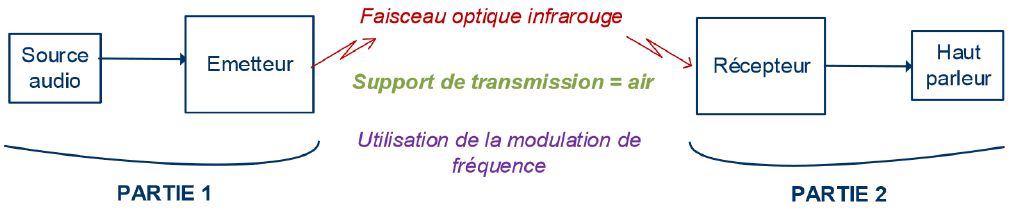
\includegraphics[width=1\textwidth]{parties.PNG}
\end{center}

\vspace{1cm}

\paragraph{} 
Ce rapport va donc détailler la conception des éléments constituant le module d’émission. La conception de chaque élément sera traitée séparément.

\paragraph{} 
On commencera par présenter le cahier des charges, puis étudier l'oscillateur contrôlé par tension\footnote{VCO}. Ensuite on exposera deux structures du VCO, l’une avec attaque en tension, la seconde avec attaque en courant, que l’on comparera pour n’en conserver qu’une  pour notre PCB. La partie suivante sera consacrée au circuit de commande de la diode électroluminescente à transistors bipolaire et à transistor MOS (MOSFET). On terminera par la conception du filtre audio d’entrée.\\



\begin{center}
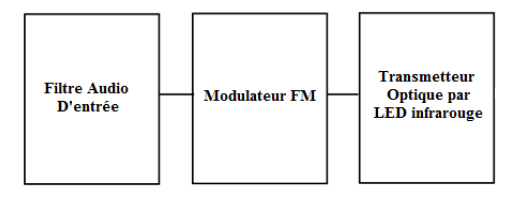
\includegraphics[width=0.7\textwidth]{bloc_emet3.PNG}
\end{center}

\part{Conception du bloc Émetteur}

$ $ 
\vspace{6cm}

L'émetteur est constitué de trois blocs : \\

\begin{center}
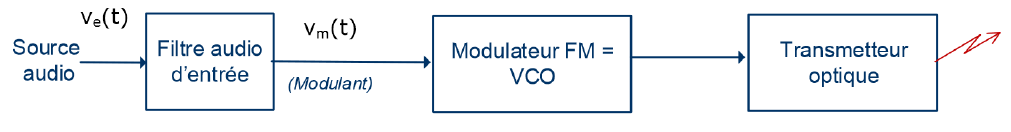
\includegraphics[width=1\textwidth]{bloc_emet.PNG}
\end{center}

\paragraph*{}

En entrée, un pré-amplificateur-filtre traite le signal modulant audio à transmettre avant de l'appliquer à la partie principale de notre bloc émetteur : le VCO. C'est lui qui va permettre de fixer la fréquence centrale $f_0$ de notre sous-porteuse, grâce à une variation linéaire de la fréquence selon la loi suivante :\\ 

$$\Delta f = K_1A_{vm}v_{ecc}$$

avec:
\begin{description}
\item	$A_{vm}$ le gain en tension de l'amplificateur audio.
\item $v_{ecc}$ l'amplitude du signal d'entrée.
\item $K_1$ gain de conversion du VCO.
\end{description}


\vspace{0.5cm}
Pour réaliser le VCO, il existe deux possibilités, structure avec une attaque en tension, avec une attaque en courant. Nous verrons les différences que ces deux possibilités apportent. Le signal modulé sera alors transmis jusqu'à une diode électroluminescente à haut rendement dont l'intensité est proportionnelle à son courant instantané de polarisation dans la plage des fréquences de modulation. Le flux lumineux émis par cette DEL sera alors transmis au bloc récepteur.\\
\vspace{0.5cm}
Nous alimenterons les transistors et AOP en +5V, afin de ne pas prendre en compte l'impact de la tension $V_{EB}$ maximale admissible des transistors.

\chapter{Cahier des charges bloc émetteur}

\section{Le filtre audio d'entrée}

Ce circuit reçoit le signal d'entrée et le transmet au VCO. Il doit satisfaire aux exigences suivantes :  
\begin{itemize}
	\item Résistance d'entrée $R_e$ = 50k$\Omega$ à la fréquence moyenne $f_m$ = 400Hz.

	\item Limiter la bande passante aux fréquences f $\in$ [50Hz ; 6kHz], et pré-accentuer sur la plage de fréquences [800 Hz ; 6kHz] afin d'optimiser le rapport signal sur bruit, en respectant le gabarit suivant:\\

\begin{center}
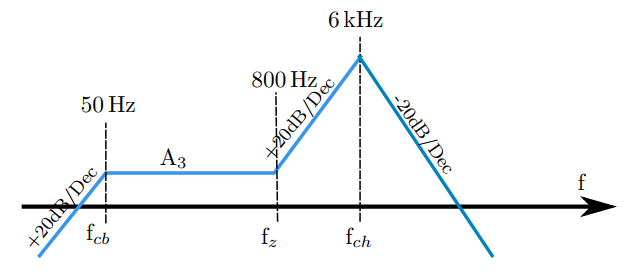
\includegraphics[width=0.8\textwidth]{gabarit.PNG}
\end{center}

	\item Permettre de régler le volume sonore grâce à un potentiomètre $P_1$ (4.7 k$\Omega$) .
	
\end{itemize}

\section{Le modulateur FM : VCO}
\paragraph{}
Le modulateur FM qui effectue donc la conversion tension-fréquence est le cœur du bloc émetteur. La modulation sera effectuée par un oscillateur commandé en tension (VCO), en respectant les critères suivants :
\begin{itemize}
\item Fréquence de la porteuse $f_0$=240kHz .
\item Présence d’un potentiomètre permettant de faire varier la fréquence de la porteuse sur une plage $\Delta f=\pm 25 \%$.
\item Pour un signal de 400 Hz on aura =7.5 kHz avec $v_e$(t)=0.5V.
\item Respecter la relation suivante:
\begin{center}
$\Delta$f = $K_1$\footnote{Le gain de conversion.}$A_{vm}$$v_{ecc}$
\end{center}
\end{itemize}


\section{l'amplificateur DEL}
\paragraph{}
Le circuit peut comporter deux composants actifs : le premier sert d'adaptateur et le second pilote la diode électroluminescente (soit CQY 89 A II de RTC, soit OD8811 Opto Diode corp). Le courant d'excitation moyen de la DEL est $I_0$ $\approx$ 50mA $\pm$20$\%$, le courant crête-à-crête sera donc de 100mA.
% * <man_lot@yahoo.com> 2017-11-18T17:03:43.205Z:
%
% ^.
Remarque :  le gain en tension $A_{vm}$ de l'amplificateur audio pour $f_m$ = 400Hz doit être tel que $\Delta f$= $\pm$7.5kHz= $K_1A_{vm}$.


\newpage
\section{Synthèse}

Voici un récapitulatif du cahier des charges de l'émetteur.\\
\begin{center}
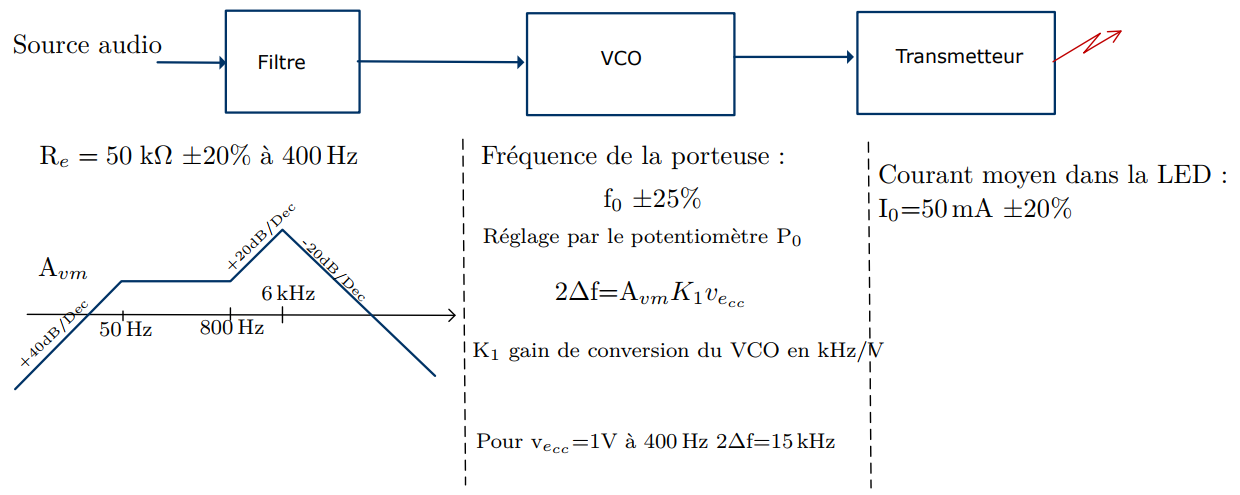
\includegraphics[width=1\textwidth]{resume.PNG}
\end{center}



\chapter{Réalisation de l'émetteur}

\section{L'oscillateur contrôlé par tension le VCO:}

\subsection{Étude du multivibrateur à couplage par collecteur}

\subsubsection{Calcul de la période des oscillations}
\begin{center}
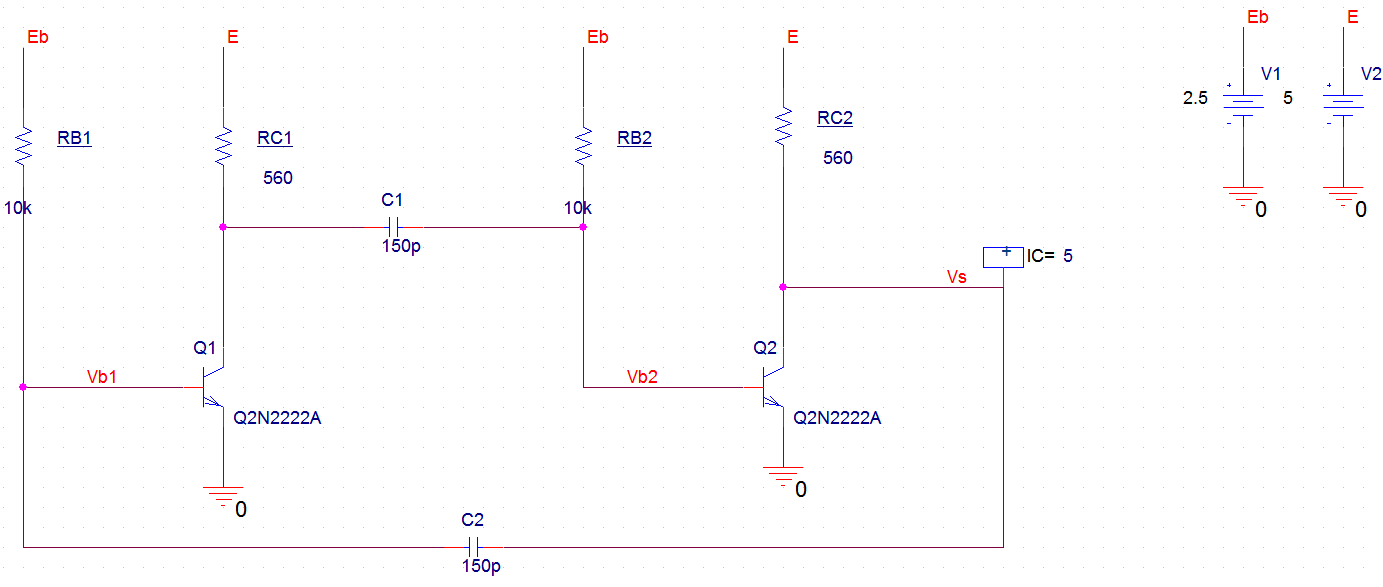
\includegraphics[width=1\textwidth]{multivib.PNG}
\end{center}


On suppose qu'à t = 0, $T_1$ est passant, et par conséquent $T_2$ est bloqué. La tension $V_{B2}$ est alors égale à $V_T$-(E-$V_{CEsat}$). \\
\vspace{0.4cm}

$\rightarrow$ Calculons dans un premier temps $R_{C1}$:

$$R_{C1} = \dfrac{E-V_{C1}}{I_{C1}} \geq \dfrac{E-V_{CEsat}}{I_{Csat}^{max}}$$

Avec: $I_{Csat}^{max}$ = 10 mA et $V_{CEsat}$ = 0.2 V (valeur lue sur la datasheet, qu'on négligera devant E afin de simplifier les calcules).\\
On trouve:
$$R_{C1} \geq 500 \Omega$$
On prendra \hspace{5.3cm} $R_{C1} = 560 \Omega$ \\

\vspace{0.5cm}
$\rightarrow$ Calculons maintenant $R_B$:\\

On a la relation:
$$I_{Bsat} > \dfrac{I_{Csat}}{\beta _{min}}$$
On prendra $\beta _{min} =60$\\

On a :
$$R_{B1}=\dfrac{\frac{E}{2}-V_{B1}}{I_{B1}}$$
Ainsi: \hspace{2.5cm} $R_{B1} < \beta _{min} \dfrac{\frac{E}{2}-V_{T}}{I_{Csat}^{max}}$ \hspace{0.6cm} donc \hspace{0.6cm} $R_{B1}<11.4k \Omega$\\

On prend:
$$R_{B1} = 10k \Omega $$

On a le circuit de charge de la capacité $C_2$ avec $T_2$ bloqué et $T_1$ saturé:\\

\begin{center}
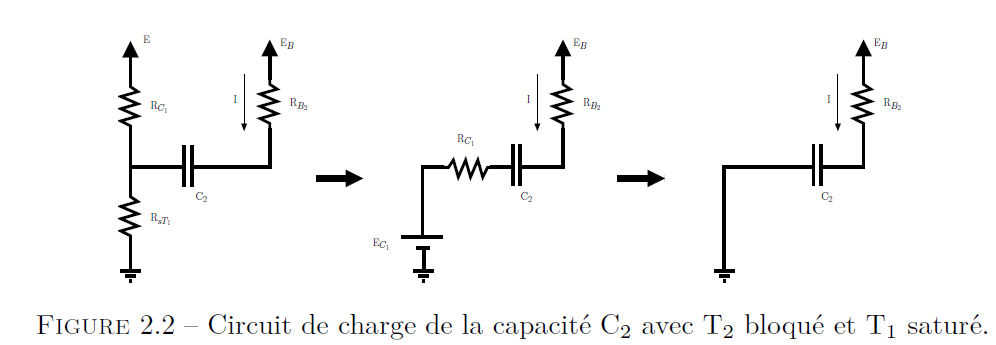
\includegraphics[width=1\textwidth]{circuitC2.PNG}
\end{center}


On a : \hspace{2cm} $V_C(0)=V_T-\left( E-V_{CEsat} \right)$ \hspace{2cm} et \hspace{2cm} $V_C(\infty)=\dfrac{E}{2}$\\

Ainsi on a l'expression de la tension aux bornes de $C_2$:

$$V_C(t)= \left( V_C(0)-\dfrac{E}{2} \right) e^{-\dfrac{t}{\tau}}+\dfrac{E}{2}$$

On en déduit: \hspace{3cm} $T_{charge}=-\tau ln \left( \dfrac{V_T-\dfrac{E}{2}}{V_C(0)-\dfrac{E}{2}} \right)$ = $\dfrac{T_{VCO}}{2}= \dfrac{1}{2f_0} = 2.1\mu s$\\
\vspace{0.2cm}
On trouve : \hspace{5cm} $C_2 = 163pF$\\
On prendra la valeur normalisée $C_2 = 150pF$\\

\vspace{0.5cm}
Par symétrie du circuit on a pris $R_{B1}=R_{B2}$, $R_{C1}=R_{C2}$ et  $ C_{1} = C_{2}$.\\

\newpage


\subsubsection{Mise en oeuvre du multivibrateur}

On a sur PSpice:
\begin{center}
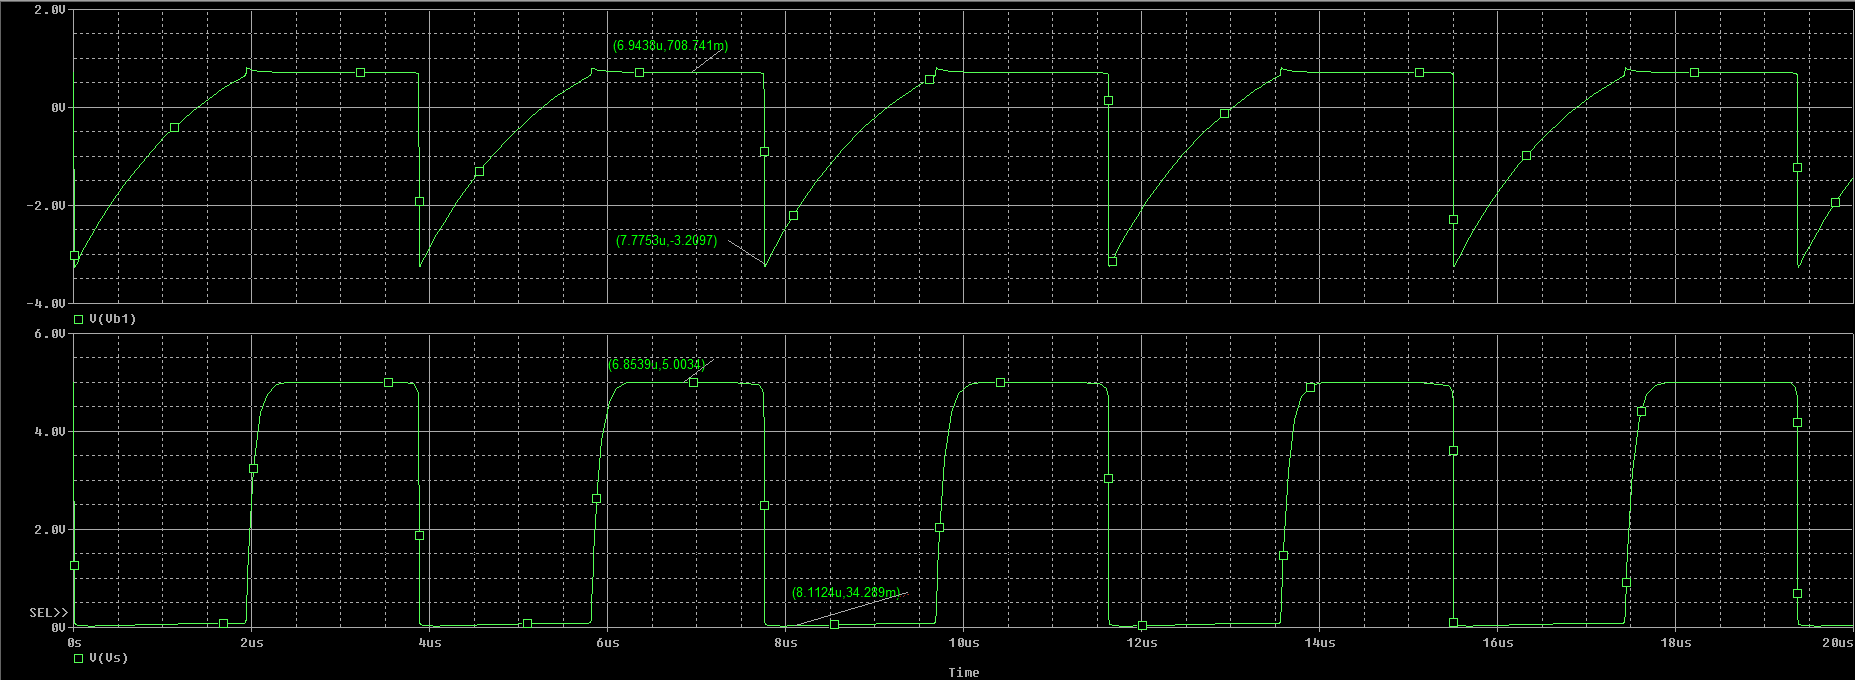
\includegraphics[width=1\textwidth]{multivib_simu.PNG}
\end{center}

On a en câblant notre montage:

\begin{center}
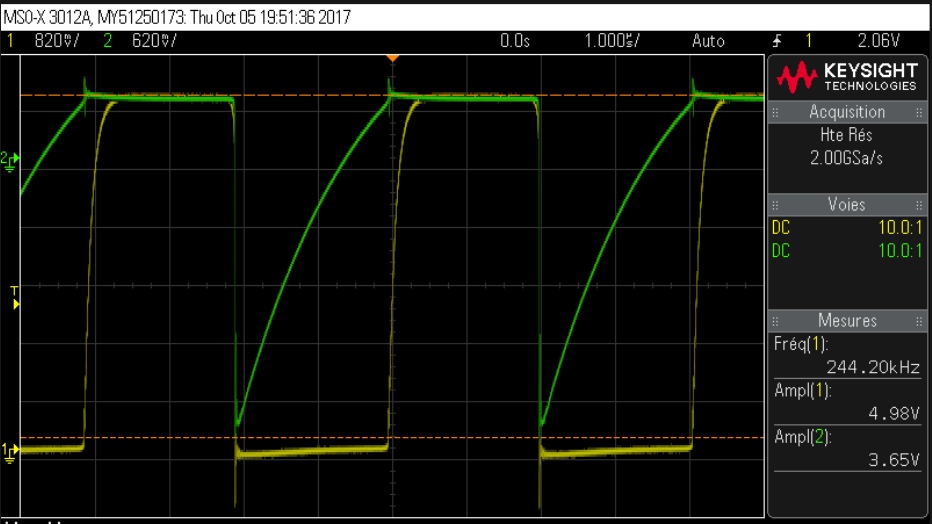
\includegraphics[width=1\textwidth]{Simu_multivib.PNG}
\end{center}

On compare maintenant nos mesures (simulation et pratique) avec nos valeurs théorique.\\

\begin{center}
\begin{tabular}{| l | c | c | c |}
\hline
 $ $ & $\Delta V_{B2}$ & $\Delta V_{C}$ & $f_T$\\
\hline
PSpice & 3.96 V & 5 V & 258 kHz   \\
\hline
Pratique & 4.3 V & 5.1 V & 244kHz   \\
\hline
Théorie & 5 V & 5 V & 258.4 kHz\footnote{En prenant en compte les valeurs normalisées des composants} \\
\hline

\end{tabular}
\end{center}
 $\rightarrow$ Impact de la capacité vue de la base du transistor : \\
 On a $\Delta V_B$ = $k\Delta V_C$. D'où :\\
 \begin{center}
 k = 0,79\\
 \end{center}

On recalcule la fréquence, on a : \\
\begin{center}
f = $\dfrac{1}{2\tau ln(\dfrac{V_T - E_B - k\Delta V_C}{V_T - E_B})}$
On obtient : f = 298,6 kHz.
\end{center}

En tenant compte du facteur k, on calcule à présent la nouvelle valeur de la période des oscillations : \\
T = $\dfrac{1}{f}$ = 3,4$\mu$s $<$ 4,2 $\mu$s : la nouvelle période est plus petite que l'ancienne, comme nous le pensions.\\


\subsection{Élaboration d'un VCO}
Dans cette partie, nous allons réaliser un oscillateur contrôlé en tension à partir du multivibrateur étudié.

\subsubsection{Structure du VCO avec Attaque en tension}

On étudie la structure suivante :

\begin{center}
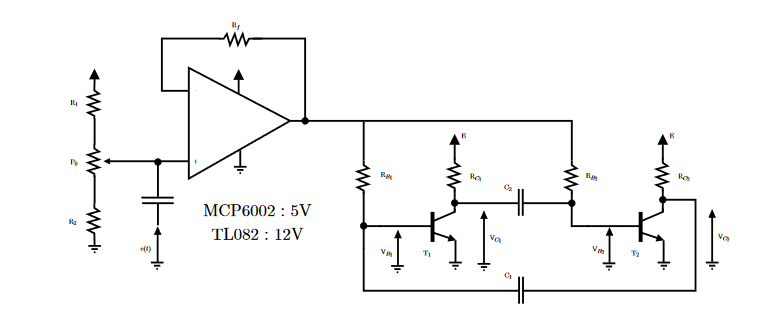
\includegraphics[width=1\textwidth]{VCO_tension.PNG}
\end{center}

On cherche à caractériser le VCO, c'est-à-dire mesurer le gain $K_1$. Pour cela, on fait varier légèrement $E_B (t)$ autour de $E/2$. On utilise le code Matlab disponible sur Moodle pour calculer la valeur théorique de $K_1$ :

\begin{center}
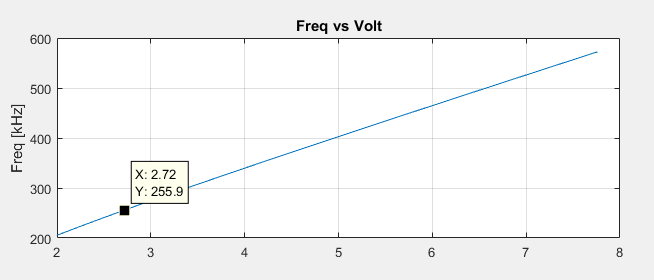
\includegraphics[width=1\textwidth]{K1_th.PNG}
\end{center}

On trouve :

\begin{center}
$K_{1th} = 77.6 kHz/V$
\end{center}

Pour calculer le $K_1$ sur PSpice, on fait varier légèrement $E_B (t)$ autour de $E/2$. On obtient ainsi la courbe suivante :

\begin{center}
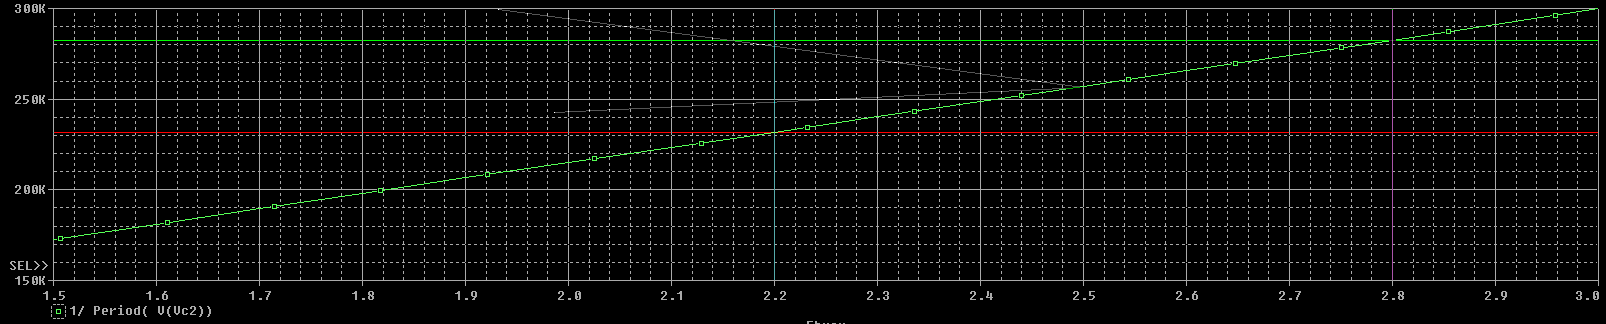
\includegraphics[width=1\textwidth]{K1_simu.PNG}
\end{center}

On trouve :

\begin{center}
$K_{1simu} = 84 kHz/V$
\end{center}

Grâce à cette courbe, on en déduit les valeurs de tension d'entrée $E_{min} = 1.9V$ et $E_{max} = 3.1V$.

Pour calculer $R_1$ et $R_2$, on "sépare" le potentiomètre en deux : $\alpha P_0$ et $(1-\alpha)P_0$. De plus, on a :

$V_+ = E_{moy} = \dfrac{(1-\alpha)P_0 + R_2}{P_0 + R_1 + R_2}.$
\\

Ainsi :
\begin{center}
$$
\left\{
    \begin{array}{ll}
        \dfrac{P_0 + R_2}{P_0 + R_1 + R_2}*E = E_{max} & \mbox{si } \alpha = 0 \\
        \dfrac{P_0}{P_0 + R_1 + R_2}*E = E_{min} & \mbox{si } \alpha = 1
    \end{array}
\right.
$$
\end{center}

On en déduit : 
\begin{center}
$$
\left\{
    \begin{array}{ll}
        R_1 = 6.8k\Omega \\
        R_2 = 6.8k\Omega
    \end{array}
\right.
$$
\end{center}

Enfin, pour la valeur expérimentale, on utilise la même méthode que sur PSpice; on obtient la courbe de $K_1$ suivante :

\begin{center}
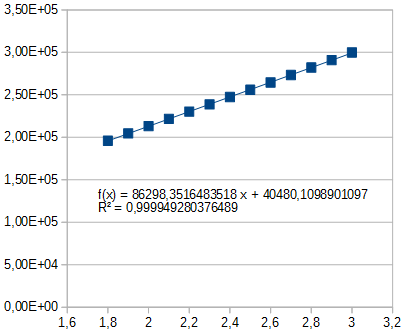
\includegraphics[width=0.5\textwidth]{K1_exp.PNG}
\end{center}

On mesure : 
$$ K_{1exp = 86.3kHz/V} $$

Enfin, on s'assure du bon fonctionnement du VCO avec la FFT de l'oscilloscope (signal modulant à 4kHz): 

\begin{center}
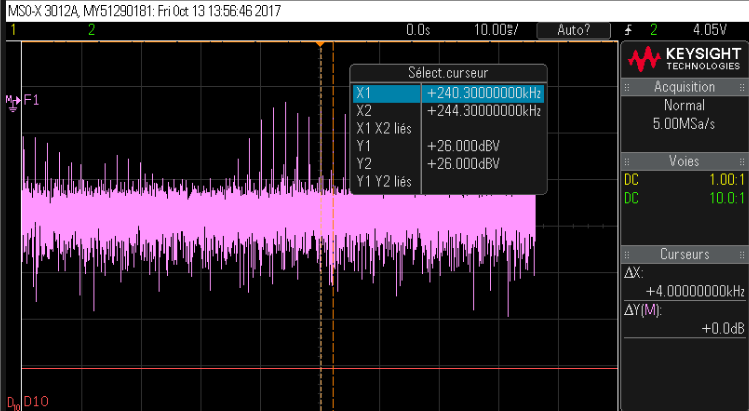
\includegraphics[width=0.7\textwidth]{fft_vco.PNG}
\end{center}

Nous sommes bien centrés en $f = 240 kHz$, avec une différence de 4kHz entre chaque pic.

\underline{Conclusion} : le VCO en attaque en tension respecte les exigences.
\newpage
\subsubsection{Structure du VCO avec Attaque en courant}

On étudie la structure suivante :

\begin{center}
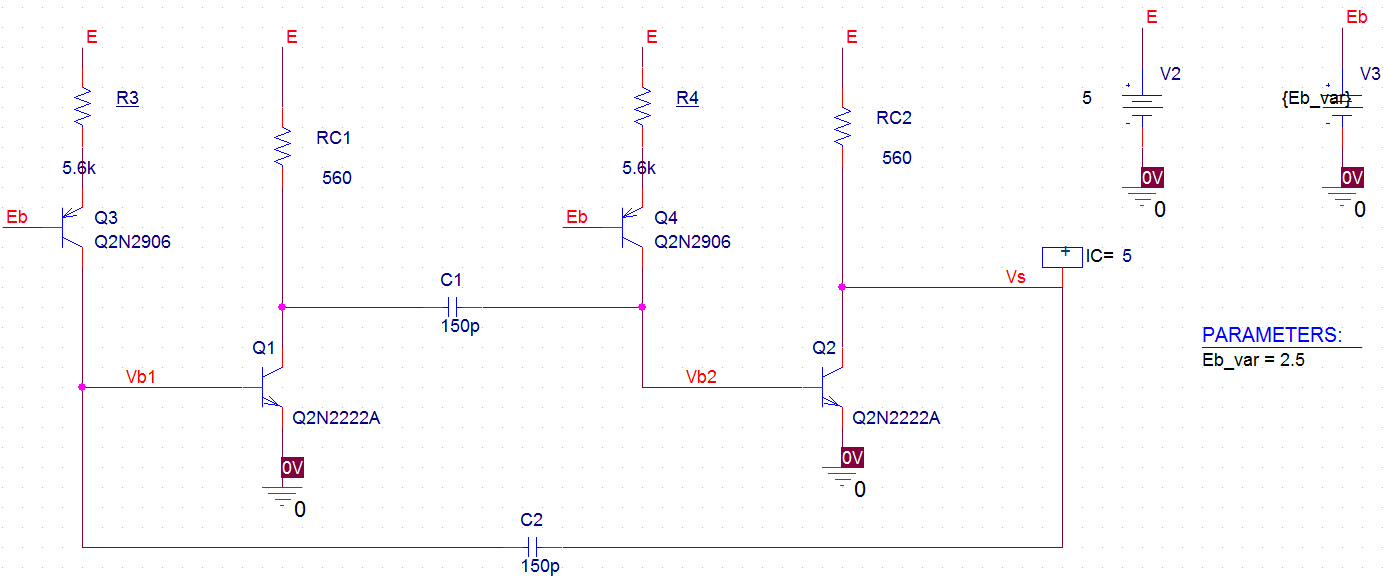
\includegraphics[width=1\textwidth]{VCOI.PNG}
\end{center}


Dans un premier temps, pour dimensionner et caractériser le VCO, on lui applique directement en entrée au niveau de la base des transistors $T_3$ et $T_4$ une tension idéale $E_B(t) = E_{moy} + e(t)$.\\
Tout d'abord on détermine la valeur du courant $I_3$ et $I_4$ pour obtenir la période $T_0$ des oscillations souhaitées pour $E_B(t) = E_{moy}$.\\
$$Schemapassur$$
On a $I_3$ qui vaut : \\
\begin{center}
$I_3 = C_1 \dfrac{dV_{C_1}}{dt} $\\
\end{center}
Or on sait que $I_3$ est constant. 
D'où :
\begin{center}
 $I_3 = C_1 \dfrac{\Delta V_{C_1}}{\Delta \tau} $
$ = C_1 \dfrac{2\Delta V_{C_1}}{T_0} $
\end{center}
On obtient donc : \\
\begin{center}
$I_3 = 3,6.10^{-4} $ A
\end{center}
De plus $I_3$ = $I_4$.\\

On cherche maintenant à exprimer $I_3$ et $I_4$ en fonction de $E_{moy}$, $R_3$, $R_4$.\\
On a :\\
$I_3 = \dfrac{E + V_{BE} - E_{moy}}{R_3}$ et $I_4 = \dfrac{E + V_{BE} - E_{moy}}{R_4}$\\
D'où :\\
\begin{center}
 $R_3 = R_4 =  \dfrac{E + V_{BE} - E_{moy}}{I_3} $\\
 $R_3 = 17,3 k\Omega$ en valeurs normalisées on a $R_3 = 18 k\Omega$
\end{center}
On a $\dfrac{I_{Csat}}{\beta _{min}} = \dfrac{10.10^{-3}}{60}= 1,67.10^{-4} A < 3,6.10^{-4} A = I_3$\\
Ce qui nous assure la saturation des transistors.\\
L'impédance de sortie de cette source de courant vaut : \\
$$ Z_S = \dfrac{V_S}{I_S} $$
$V_S = (I_S + g_mV_b) r_{ce} + R_3I_3 = (I_S + I_3  \beta^2) r_{ce} + R_3I_3 $\\
$I_S = I_3(1+\beta)$\\
D'où $Z_S = 27,3 M\Omega$\\
Cette valeur nous assure le bon fonctionnement du multivibrateur.

On a une variation du $V_{C}$ entre $V_{BE}$
et $V_{BE}-\Delta V_C$\\
Ce qui implique une variation du $V_{CE}$ entre $V_{BE}-V_e$ et $V_{BE}-\Delta V_C-V_e$
avec $V_e=E-R_3I_3$\\
Et donc $V_{CE} \in [ -2.52 ; -7.528 ] V $ \\
On respecte la limite imposée sur la DataSheet à savoir $V_{CE}>-60V$ \\

Sous Pspice, on fait varier $E_B$ autour de $\dfrac{E}{2}$ et on trace la caractéristique de notre VCO. On obtient : \\
\begin{center}
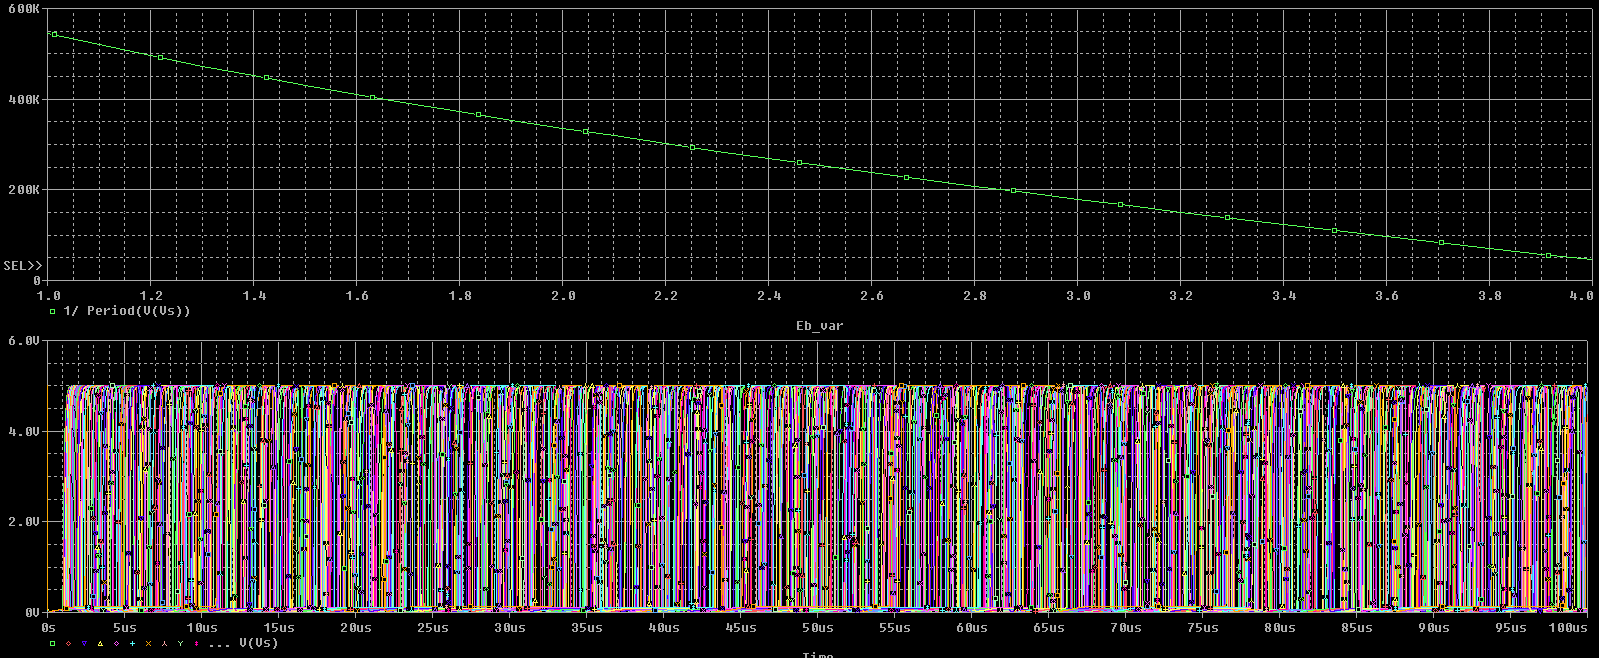
\includegraphics[width=1\textwidth]{attaque_c_vco-eb.PNG}
\end{center}

Le gain de conversion $K_1$ qui est la pente de la droite est de $1,56.10^5$ autour de la fréquence centrale $f_0$.\\

On cherche maintenant à exprimer $K_1$ théoriquement.\\
D'une part on sait que :
\begin{center}
 $I_3 = C_1 \dfrac{dV_c}{dt}$ = $\dfrac{(E-
V_{CEsat})2C_1}{T_0}$ = $(E-V_{CEsat})2C_1f_0$
\end{center}

D'autre part on a : \\
$$I_3 = \dfrac{E+V_{BE}-E_{moy}}{R_3}$$
D'où : \hspace{4cm} $f_0 = \dfrac{E+V_{BE}-E_B}{2R_3C_1(E-V_{CEsat})} $\\
Or,\hspace{5cm} $K_1$ = $\dfrac{-df_0}{dE_B}$\\
D'où \hspace{4cm} $K_1$ = $\dfrac{1}{2R_3C_1(E-V_{CEsat})}$.\\ 
On trouve $K_1$ = $1,19.10^5$.\\
La caractéristique de notre VCO est linéaire de 218kHz à 280kHz.\\

$$Avantage$$

On cherche maintenant à réaliser la source $E_B(t)$. Pour cela on utilise un potentiomètre $P_0$ et un pont diviseur de tension.\\
\begin{center}
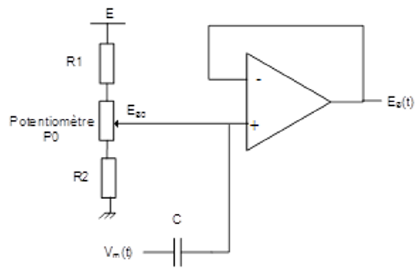
\includegraphics[width=.5\textwidth]{POT.PNG}
\end{center}

Le potentiomètre permet de régler les erreurs liées à la normalisation des valeurs.\\
On modélise le potentiomètre par deux résistances : \\
$$Schema$$
On a donc : \\
\begin{center}
$E_{moy}$ = $ \dfrac{(1+\alpha)P_0 + R_2}{P_0 + R_1 + R_2} E$\\
\end{center}
On veut $E_{moy}$ = $\dfrac{E}{2}$\\
Pour $\alpha = 0$ on a : \\
\begin{center}
$\dfrac{P_0 + R_2}{P_0 + R_1 + R_2} = \dfrac{E_{Bmax}}{2} = \dfrac{5}{8}$\\
\end{center}
Et pour $\alpha = 1$ on a : \\
\begin{center}
$\dfrac{R_2}{P_0 + R_1 + R_2}= \dfrac{E_{Bmin}}{2} = \dfrac{3}{8}$\\
\end{center}

En faisant le rapport des deux on obtient : \\
\begin{center}


 $\dfrac{P_0 + R_2}{R_2}$ = $\dfrac{5}{3}$ \\
\end{center}
D'où : \\
\begin{center}
$R_2$ = $\dfrac{3P_0}{2}$ = $7,05k \Omega$ et $R_1$ = $\dfrac{5R_2}{3}-P_0$ = $6,6k \Omega$\\
\end{center} 
On prend $R_1$ = $R_2$ = $6.8k \Omega$.\\
On peut modéliser ce circuit à l'aide d'une représentation de Thévenin avec $E_{TH}$ et $R_{TH}$.\\
On a le schéma suivant :\\
\begin{center}
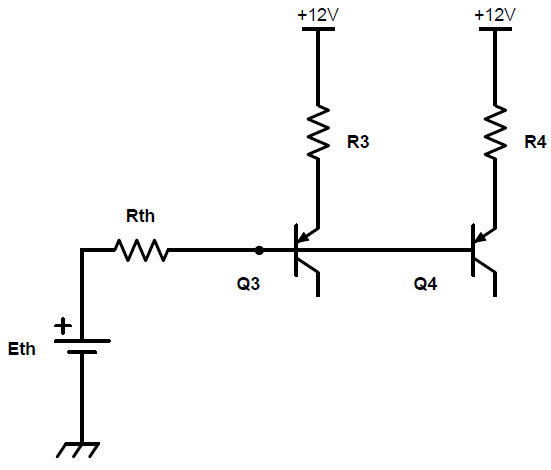
\includegraphics[width=.41\textwidth]{th.PNG}
\end{center}
On obtient donc : \\
\begin{center}
$E_{TH}$ = $\dfrac{R_2 + (1-\alpha)P_0}{P_0 + R_1 + R_2}E$ et $R_{TH}$ = $(R_1 + \alpha P_0)//(R_2 + (1-\alpha)P_0)$ = $4,27k\Omega$\\
\end{center}
On a $I_3$ = $\dfrac{E-V_{EB}-E_{TH}}{\dfrac{R_{TH}}{\beta}+ R_3}$\\
Pour avoir un courant $I_3$\footnote{respectivement $I_4$} indépendant du gain $\beta$ il faut que $\dfrac{R_{TH}}{\beta} \ll R_3$.

$$Valeur de C$$

\subsection{Caractérisation du VCO}
Dans un premier temps on cherche à mesurer le facteur k. On sait que $k=\dfrac{\Delta V_B}{\Delta V_C}$.
On mesure $\Delta V_B$ = 3,88V et on a $\Delta V_C$ = 5V. On en déduit k = 0,776.\\
On trace, sur MATLAB, $f_VCO$ en fonction de la tension de commande, on a : \\
\begin{center}
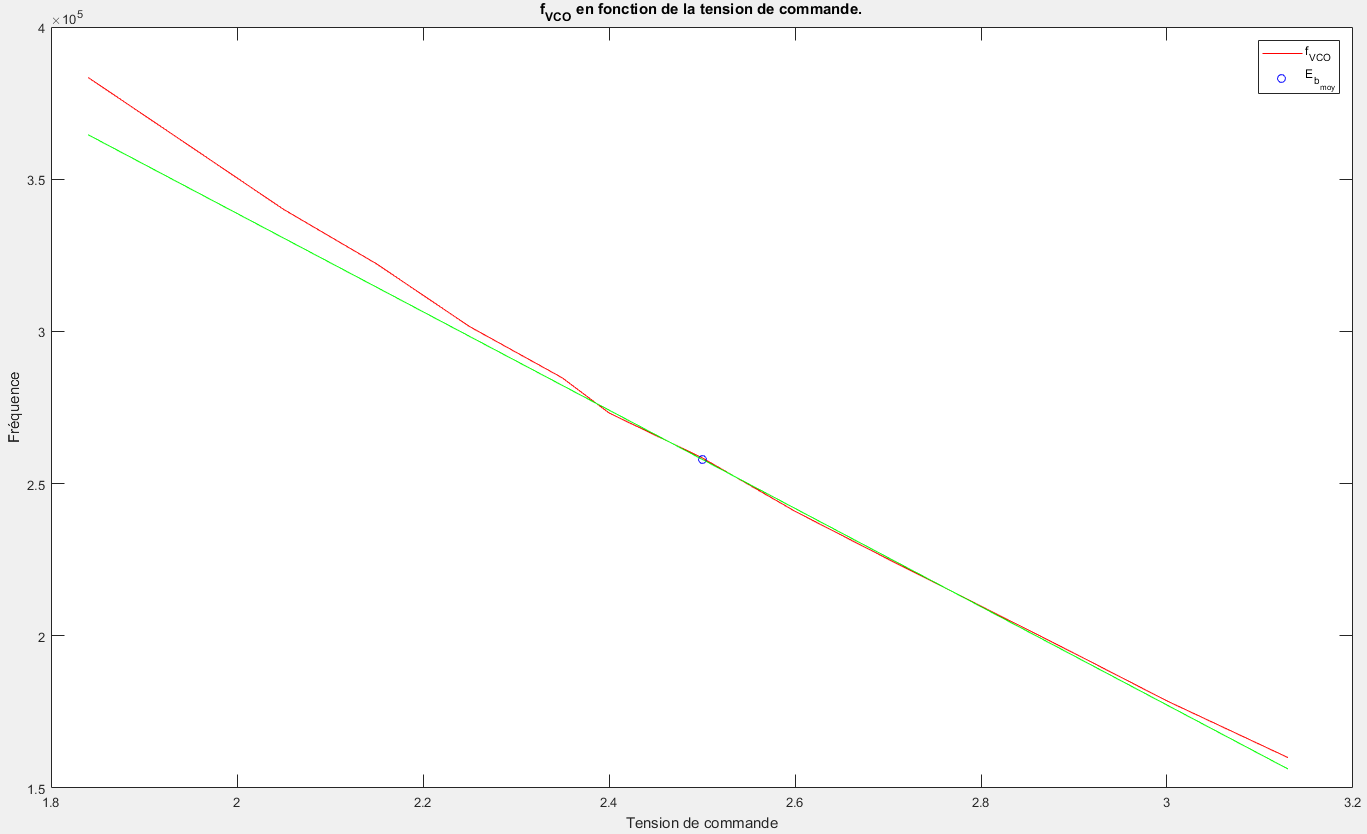
\includegraphics[width=1\textwidth]{fvco.PNG}
\end{center}
On mesure $K_1$ autour de la fréquence centrale $f_0$, on obtient : \\
La droite en vert nous permet de délimiter la zone de linéarité de la caractéristique du VCO autour de $f_0$.
\begin{center}
$K_1$ = $\dfrac{-(240,9-273,2).10^3}{2.6-2.4}$ = $1,615.10^5$\\
\end{center}
Nous avons commencé par concevoir le VCO car celui-ci possède un gain $K_1$ non négligeable. En effet, nous avons la relation suivante : \\
\begin{center}
$2\Delta f = K_1 A_{vm} V_{ecc}$
\end{center}
Ainsi il était nécessaire de connaître $K_1$ avant de dimensionner le filtre audio.\\
\section{Circuits de commande de la diode électroluminescente}
Pour nos modélisations Pspice on utilise la diode DBREAK de la bibliothèque BREAKOUT. Pour savoir quels sont les paramètres à entrer on utilise les données constructeurs.\\
$R_S$ représente l'inverse de la pente de la caractéristique $I_F=f(V_F)$ qui est donnée par le constructeur.\\ On a donc $R_S$ = $\dfrac{1,4 - 1,3}{(100-50).10^{-3}}$ = 2$\Omega$\\
Le courant $I_S$ se calcule à partir de la relation $I_F$ = $I_S(e^{\dfrac{V_F}{nU_T}}-1)$ pour $I_F$ = 100mA.\\ On obtient $I_S$ = $4,88.10^{-16}$\\
La valeur du condensateur $C_{j0}$ est de 40pF.

\subsection{Transmetteur à Transistor Bipolaire}
On étudie la structure suivante : 

\begin{center}
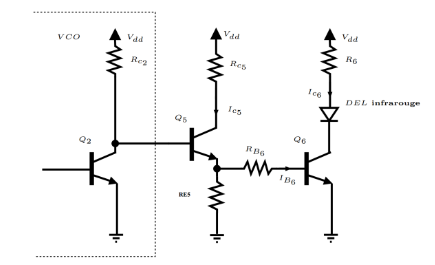
\includegraphics[width=0.6\textwidth]{montage_diode.PNG}
\end{center}

\subsubsection{Dimensionnement de $Q_6$}

On dimensionne dans un premier temps $Q_6$.

D'après les datasheet, la tension de seuil $V_F$ de la DEL lorsqu'elle est parcourue par un courant de $I_0 = 100mA$ est  $V_f = 1.4 V$ ; la tension maximale de saturation de $Q_6$ est $V_{CEsat} = 0.4 V$.

Par une loi des mailles, on a : 
$$ V_{dd} = V_{CEsat} + V_F + I_{C6}R_6$$
On en déduit : $$R_{B6} = 33\Omega$$

$P_{R6} = \dfrac{R_6 I_0^{2}}{2} = 0.17 W$

Il faut utiliser un boîtier $\dfrac{1}{4}W.$\\

Pour déterminer $R_{B6}$, on se place dans le cas où $Q_6$ est saturé :\\
$\beta_{min} I_{B6} > I_{C6}$\\
$I_{B6} > 2mA$\\
$R_{B6} = \dfrac{V_{R_{B6}}}{I_{R_{B6}}}$ avec $V_{R_{B6}} = E - V_{BE5} - V_{BE6}$\\
Ainsi : $$R_{B6} = 2.2k\Omega$$

\subsubsection{Amélioration du temps de commutation de $Q_6$}
On caractérise le temps de commutation ON et OFF du transistor $Q_6$ en ne câblant que $Q_6$ avec $R_6$ et $R_{B6}$. A l'aide de l'annexe, on mesure/calcule les temps des différentes phases de commutation de $Q_6$ (i.e. diminuer $t_r$).

On trouve :
$$t_f = 29ns$$
$$t_s = 30ns$$
$$t_d = 350ns$$
$$t_r = 180ns$$

\begin{center}
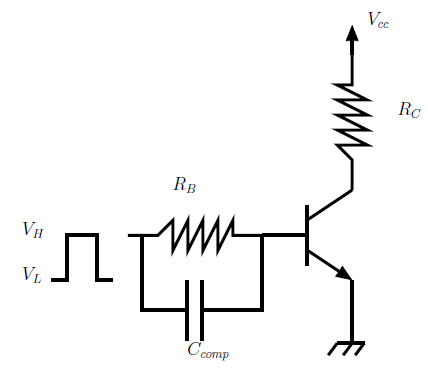
\includegraphics[width=0.4\textwidth]{commutation_Q6.PNG}
\end{center}

$C_{comp}$ sert à diminuer le temps de commutation de $Q_6$.\\
On a $$C_{comp} = \dfrac{\tau_S}{R_{B6}}$$
avec $\tau_s = \dfrac{t_s}{ln(\dfrac{I_{Bon}-I_{Boff}}{I_{Blim}-I_{Boff}})} = 92.2ns$\\

On trouve : $$C_{comp} = 47pF$$

\subsubsection{Dimensionnement de $Q_5$}

On pose $I_{RE5} = I_{RB6}$ pour simplfifer les calculs. On a :
$$r_5 = R_{E5} // (\dfrac{u_t}{I_{C5}} + \dfrac{R_{C2}}{\beta_5})$$
Le deuxième terme en parallèle avec $R_{E5}$ est l'impédance de sortie de $Q_5$. Ainsi, on veut $R_{E5} >> 16\Omega$. Pour avoir de la marge, on prend : 
$$R_{E5} = 1.8k\Omega$$.
$R_{C5}$ a un rôle de protection. On prend :
$$R_{C5} = 50\Omega$$

\subsubsection{Etude du rémine transistoire du transmetteur optique}

On place la DEL en sortie de $Q_6$.

On mesure dans un premier temps, à l'aide du circuit transimpédance, le temps de montée globale $t_{r_{s}}$ de la chaîne.

On obtient :

\begin{center}
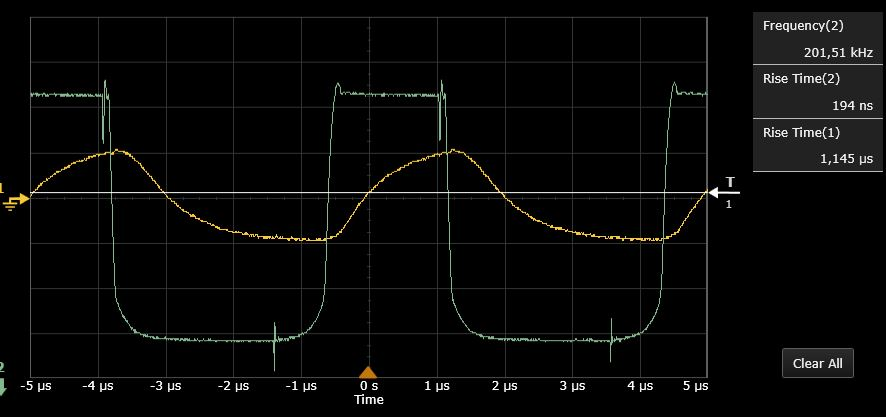
\includegraphics[width=1\textwidth]{trs.JPG}
\end{center}

$$t_{r_{s}} = 1.145 \mu s$$

On mesure maintenant $t_{r_{i}}$ aux bornes de $R_6$ en mode AC. On obtient :

\begin{center}
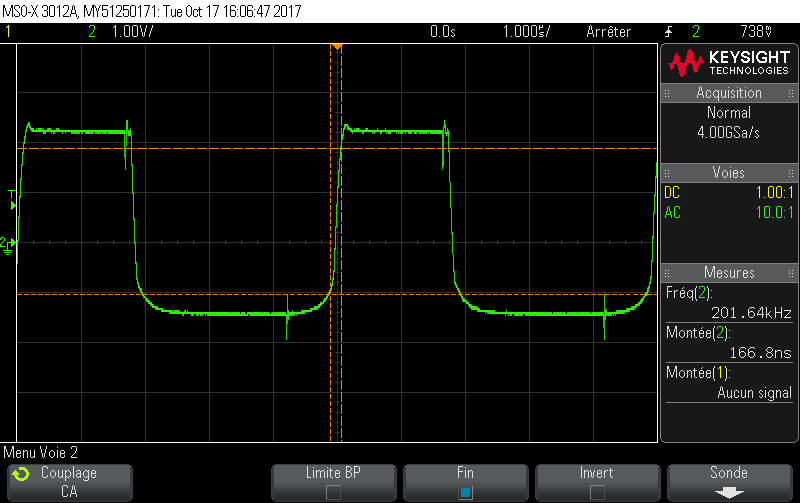
\includegraphics[width=1\textwidth]{tri_ac.png}
\end{center}

$$t_{r_{i}} = 166.8 ns \mu s$$

Enfin, le circuit transimpédance possède une fréquence de coupure haute $f_{chf} = 1.2MHz$. Le temps de montée associé à cette fréquence est $t_{r_{z}} = \dfrac{0.35}{f_{chf}}$.\\

On obtent :

$$t_{r_{z}} = 292ns$$

A partir de ces 3 temps, on en déduit le temps de montée global de la chaîne :

$$t_{r_{sth}} \approx 1.1*\sqrt{t_{rDEL}^2 + t_{r_{i}}^2 + t_{r_{z}}^2} \approx 664ns$$

On remarque que l'on a $t_{r_{sth}} \approx \dfrac{t_{r_{s}}}{2}$

\subsubsection{Amélioration du temps de montée $t_{r_{DEL}}$}

Pour améliorer $t_{r_{DEL}}$, on place une résistance et une capacité (en série) en parallèle de la résistance $R_6$ comme sur le schéma ci-dessous :

\begin{center}
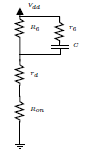
\includegraphics[width=0.15\textwidth]{montage_amelio_trdel.PNG}
\end{center}

On peut écrire :

$$I(p) = \dfrac{E-V_F}{p}\dfrac{1+\tau_1p}{R_{eq}(1+\tau_2p)}$$

avec :
\newline
\newline
$\left\{
\begin{array}{l}
  R_0 = r_d + R_{on}\\
  R_{eq} = R_0 + R_6\\
  \tau_1 = C(r_6+R_6)\\
  \tau_2 = C(R_6r_6 + R_0(r_6+R_6))
\end{array}
\right.$
\newline
\newline
De plus, le flux lumineux est lié au courant par la relation suivante : 

$$\Phi(p) =I(p) \dfrac{k}{1+\tau_0p}$$

On cherche  à ce que $\tau_1$ compense $\tau_0$, soit $\tau_1 = \tau_0$.
$\tau_0$ est donné par $\tau_0 = \dfrac{t_{r_{DEL}}}{2.2}$ avec $t_{r_{DEL}} = 0.5\mu s$.
Ainsi, on a : $C(r_6+R_6) = 227ns$.\newline

\underline{Détermination de $r_6$} :\newline

A $t = 0^+$, $i(0^+) = I_{F_{max}} = \dfrac{E-V_F}{r_6//R_6 + r_d + R_{on}}$ avec :\newline
\newline
$\left\{
\begin{array}{l}
  R_{on} = 4\Omega\\
  r_d = 1.5\Omega \mbox{    d'après la datasheet}\\
\end{array}
\right.$
\newline
\newline
On fait l'hypothèse que $r_6<<R_6$. On obtient une valeur théorique de $r_6$ de $33\Omega$, mais pour limiter le courant traversant $r_6$ et avoir un meilleur résultat, on prend :

$$r_6 = 10\Omega$$

On en déduit :

$$C = 63nF$$

On met en place le montage suivant :

\begin{center}
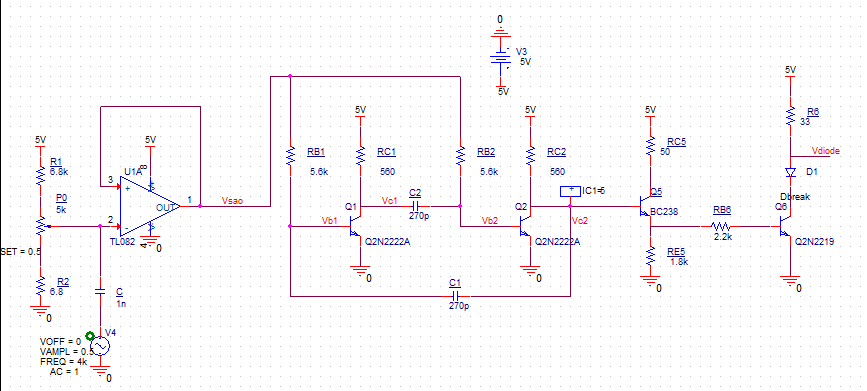
\includegraphics[width=1\textwidth]{Montage_DEL.PNG}
\end{center}

et on additionne le courant traversant $R_6$ et celui traversant $r_6$. On obtient :

\begin{center}
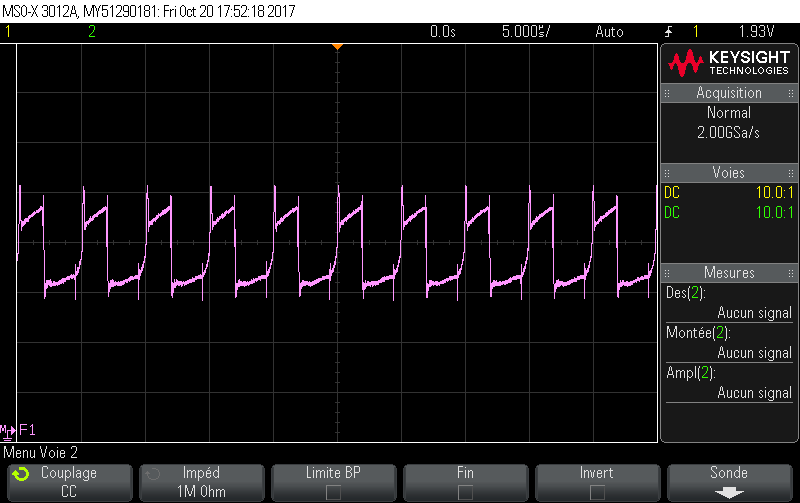
\includegraphics[width=1\textwidth]{Courant_diode_opt.png}
\end{center}



\subsection{Transmetteur à Transistor MOS}
On étudie la structure suivante : \\
\begin{center}
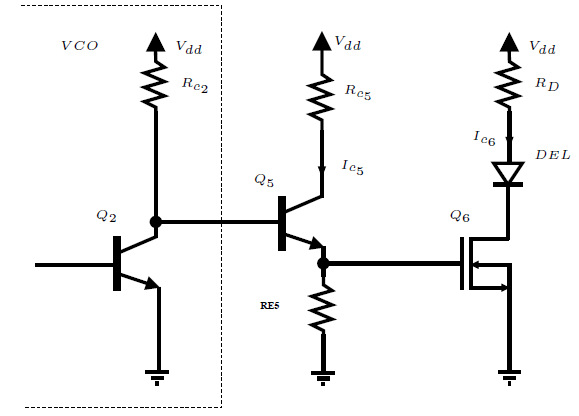
\includegraphics[width=.5\textwidth]{transimos.PNG}
\end{center}

En théorie, le transistor $Q_5$ n'est pas nécessaire. En effet le transistor MOS se comporte comme un condensateur en entrée alors que le transistor bipolaire nécessite une adaptation car il s'apparente à une résistance.\\

D'après la datasheet on a la tension de seuil $V_F$ = 1,4V lorsqu'elle est parcourue par un courant $I_0$ = 100mA.\\
On cherche maintenant la résistance $R_{DSon}$ du transistor pour une tension de commande de 5V, on a $R_{DSon}$ = 1,8 $\Omega$. On peut donc en déduire $R_D$ :\\
On a $(R_S + R_{DSon} + R_D) I_0 = V_{dd}$\\
D'où $R_D$ = $\dfrac{V_{dd}}{I_0} - R_S -R_{DSon}$ = $46,2 \Omega$\\
On calcule la puissance que doit dissiper la résistance $R_D$ afin de savoir quel type de boîtier nous devrons utiliser.\\
On a : $2P = UI_0$ = $R_DI_0^2$ = 0,462 W. Il faut donc utiliser un boîtier qui permet de dissiper une puissance $\dfrac{1}{4}W$.\\
On cherche maintenant à caractériser la commutation à l'état ON et OFF du transistor MOS en ne câblant que $Q_6$ avec une résistance de grille $R_G$ dont la valeur est égale à l'impédance de sortie du VCO ce qui permet de remplacer le VCO par cette résistance lors des tests de la DEL.
$$Circuit_test_commu$$
Pour cela on mesure les différents temps correspondants aux différentes phases en utilisant l'annexe F, on a le temps d'allumage donné par :  $t_{on} = t_2 + t_3$. On cherche donc $t_2$ et $t_3$ :  \\
\begin{center}

$t_2$ = - $R_G$ ($C_{GS} + C_{GD}$) $ ln(1-\dfrac{V_{GP}}{V_G}$)
$t_3$ = $C_{GD}R_G$ $\dfrac{V_{dd}}{V_G - V_{GP}}$

\end{center}
On prend $V_{GP}$ = 3.2 V ( lecture sur le graphique de la datasheet ) et $V_G$ = 5V.\\
$$Datasheet$$
On trouve $t_2$ = 20 ns et $t_3$ = 7 ns, ce qui donne $t_{on}$ = 27 ns.
Pour calculer le temps de montée $t_r$ = $t_2 - t_1$ on calcule $t_1$. Pour cela on réutilise la formule pour $t_2$ en prenant $V_{GP}$ = 2.1V. On trouve $t_1$ = 10.6 ns. D'où $t_r$ = 9.4 ns.\\
On câble maintenant la DEL. On obtient : \\
$$photo$$
On cherche maintenant à comparer les temps mesurés, théoriques et simulés : \\
\begin{center}
\begin{tabular}{| l | c | c | c | c | c |}
\hline
 $$ & $t_1$ & $t_2$ & $t_3$ & $t_{on}$ & $t_r$\\
\hline
Théorie & 10.6 n & 20 n & 7 n & 27 n & 9.4 n   \\
\hline
Simulation  & x & x & x & 35 n & x   \\
\hline
Pratique  & 19 n & 24 n & 45 n & 69 n & 5 n  \\
\hline
\end{tabular}
\end{center}
Le transistor MOSFET n'est pas réaliste, il monte directement à 2V, comme s'il était chargé à courant constant, ce qui permet d'expliquer les importantes différences.

On souhaite mesurer à l'aide du circuit transimpédance le temps de montée global $t_{rs}$ de la chaîne en faisant attention à ne pas saturer le signal de sortie du transimpédance en plaçant le récepteur optique à une distance "raisonnable" de la DEL d'émission. On obtient : \\
$$sansrc$$
D'où $t_{rs}$ = 1.0 $\mu$ s.\\
On mesure $t_{ri}$ aux bornes de $R_6$, on obtient $t_{ri}$= 38 ns. Dans la datasheet on trouve 20 ns, ce qui est plus ou moins cohérent.\\
Le temps de montée associé à la décroissance du $1^{er}$ ordre aux hautes fréquences avec une fréquence de coupure $f_{chf}$ = 1.2 MHz est : 
\begin{center}
$t_{rz}  = \dfrac{0.35}{f_{chf} } = 2.92.10^{-7} s$

\end{center}

On a : \\
\begin{center}
$t_{rs} \approx 1.1 \sqrt{t_{rDEL}^2 + t_{ri}^2 + t_{rz}^2 } $
\end{center}
Avec : \\
$t_{rDEL} = 0.5 \mu s$ ;\\
$t_{ri} =38 ns$ ; \\
$ t_{rz} = 2.92.10^{-7}s$ .\\
D'où $t_{rs} = 0.64 \mu  s$.
On a un rapport de $\dfrac{2}{3}$ entre $t_{rsMesure}$ et $t_{rsCalcul}$, ce qui est normal.\\
On cherche maintenant à réduire ce temps de montée or, comme les temps de montée s'additionnent au carré, c'est la valeur la plus importante qui impose le résultat final. Ainsi pour diminuer $t_{rs}$ il faut réduire $t_{rDEL}$.\\


Pour cela, on place une résistance et une capacité (en série) en parallèle de la résistance $R_6$ comme sur le schéma ci-dessous :

\begin{center}
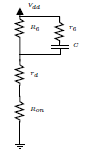
\includegraphics[width=0.15\textwidth]{montage_amelio_trdel.PNG}
\end{center}

On peut écrire :

$$I(p) = \dfrac{E-V_F}{p}\dfrac{1+\tau_1p}{R_{eq}(1+\tau_2p)}$$

avec :
\newline
\newline
$\left\{
\begin{array}{l}
  R_0 = r_d + R_{on}\\
  R_{eq} = R_0 + R_6\\
  \tau_1 = C(r_6+R_6)\\
  \tau_2 = C(R_6r_6 + R_0(r_6+R_6))
\end{array}
\right.$
\newline
\newline
De plus, le flux lumineux est lié au courant par la relation suivante : 

$$\Phi(p) =I(p) \dfrac{k}{1+\tau_0p}$$

On cherche  à ce que $\tau_1$ compense $\tau_0$, soit $\tau_1 = \tau_0$.
$\tau_0$ est donné par $\tau_0 = \dfrac{t_{r_{DEL}}}{2.2}$ avec $t_{r_{DEL}} = 0.5\mu s$.
Ainsi, on a : $C(r_6+R_6) = 227ns$.\newline

\underline{Détermination de $r_6$} :\newline

A $t = 0^+$, $i(0^+) = I_{F_{max}} = \dfrac{E-V_F}{r_6//R_6 + r_d + R_{on}}$ avec :\newline
\newline
$\left\{
\begin{array}{l}
  R_{on} = 1.8\Omega\\
  r_d = 14\Omega \mbox{    d'après la datasheet}\\
\end{array}
\right.$
\newline
On fait l'hypothèse que $r_6<<R_6$. On obtient une valeur théorique de $r_6$ de $33\Omega$, mais pour limiter le courant traversant $r_6$ et avoir un meilleur résultat, on prend :

$$r_6 = 10\Omega$$

On en déduit :

$$C = 63nF$$

On met en place le montage suivant :

\begin{center}
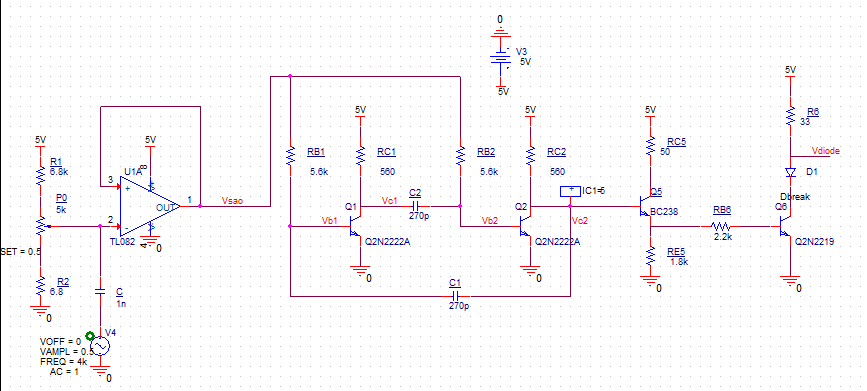
\includegraphics[width=1\textwidth]{Montage_DEL.PNG}
\end{center}

et on additionne le courant traversant $R_6$ et celui traversant $r_6$. On obtient :

\begin{center}
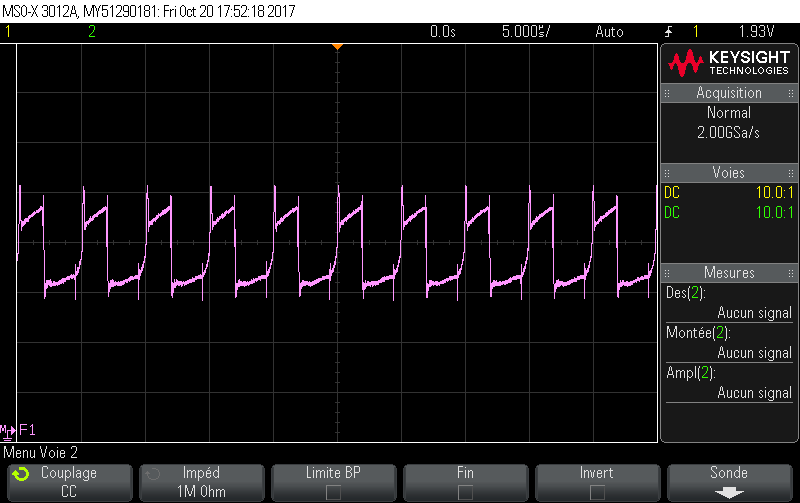
\includegraphics[width=1\textwidth]{Courant_diode_opt.png}
\end{center}
\newpage
\chapter{Filtre audio d'entrée}

Ce circuit permet de recevoir le signal audio à transmettre et d'effectuer un filtrage de pré-accentuation. Le gabarit du filtre est donné sur la figure ci-dessous :

\begin{center}
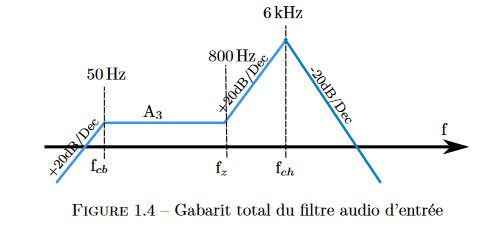
\includegraphics[width=0.7\textwidth]{gabarit_total.PNG}
\end{center}

\section{Etude théorique}

Pour réaliser le filtre audio, on utilise la structure suivante :

\begin{center}
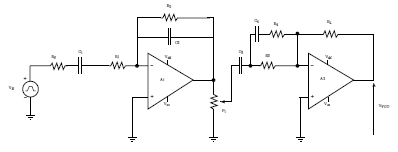
\includegraphics[width=1\textwidth]{montage_filtre_audio.PNG}
\end{center}

\subsection{Calcul de $A_{vm}$}

On a la relation suivante :

$$\Delta f = A_{vm}K_1V_{cc}$$

avec :\\


$\left\{
\begin{array}{l}
  \Delta f = 15kHz\\
  V_{cc} = 1V\\
  K_1 = 86.3kHz/V
\end{array}
\right.$

On en déduit : 
$$A_{vm} = 0.0229$$

\subsection{Calcul des valeurs des composants}

\textbf{\underline{Remarque}} :
\newline
\newline
$C_3$ sert à filtrer la composante continue de $v_{s1}(t)$, on ne la prend pas en compte dans la détermination des fonctions de transert des deux étages. 
\newline
\newline

La fonction de trasnsfert du 1er étage est donnée par :

$$H_1(p) = \dfrac{-R_2C_1p}{(1+R_1C_1p)(1+R_2C_2p)}$$

On a de plus les relations suivantes :
\newline
\newline
$\left\{
\begin{array}{l}
  Z_e = \sqrt{R_1^2 + (\dfrac{1}{2\pi f_{c1}})^2} \approx R_1 \\
  f_{cb} = \dfrac{1}{2\pi R_1C_1}\\
  f_{ch} = \dfrac{1}{1\pi R_2C_2}
\end{array}
\right.$
\newline
\newline
Le cahier des charges nous impose $Z_e = 50k\Omega$, on en déduit :

$$R_1 = 47k\Omega$$
$$C_1 = 68nF$$

De plus, on prend $R_2$ de façon à faire coïncider les fréquences de coupure introduites par $R_2C_1p$ et $R_2C_2p$.

Pour le premier étage, on a donc \\
$$\left\{
\begin{array}{l}
  R_1 = 47k\Omega\\
  R_2 = 47k\Omega\\
  C_1 = 68nF\\
  C_2 = 560pF
\end{array}
\right.$$

La fonction de transfert du 2è étage est donnée par :

$$H_2(p) = \dfrac{-R_5}{R_3}\dfrac{1+C_4p(R_3+R_4)}{1+R_4C_4p}$$

Ainsi :

$$|A_{vm}| = \dfrac{R_5}{R_3}$$

On pose :

$$\left\{
\begin{array}{l}
  R_4C_4 = \dfrac{1}{2\pi f_{ch}}\\
  C_4(R_3+R_4) = \dfrac{1}{2\pi f_z}\\
  R_3 = \dfrac{1}{2\pi C_3f_{cb}}\\
  f_z = 50Hz
\end{array}
\right.$$
\newline
\newline

Ainsi, on a toutes les valeurs des composants du filtre audio :


$$\left\{
\begin{array}{l}
  R_1 = 47k\Omega\\
  R_2 = 47k\Omega\\
  C_1 = 68nF\\
  C_2 = 560pF\\
  R_3 = 3.3k\Omega\\
  R_4 = 470\Omega\\
  R_5 = 560\Omega\\
  C_3 = 1\mu F\\
  C_5 = 56nF
\end{array}
\right.$$
\newline
\newline

\section{Mise en \oe uvre des résultats}

On teste le montage suivant :

\begin{center}
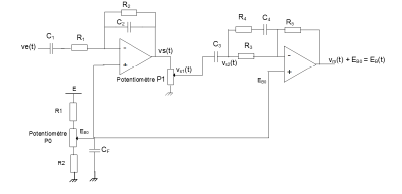
\includegraphics[width=1\textwidth]{montage_filtre_audio_complet.PNG}
\end{center}

\subsection{Simulation du filtre audio}

On trace le diagramme de Bode sous PSpice :

\begin{center}
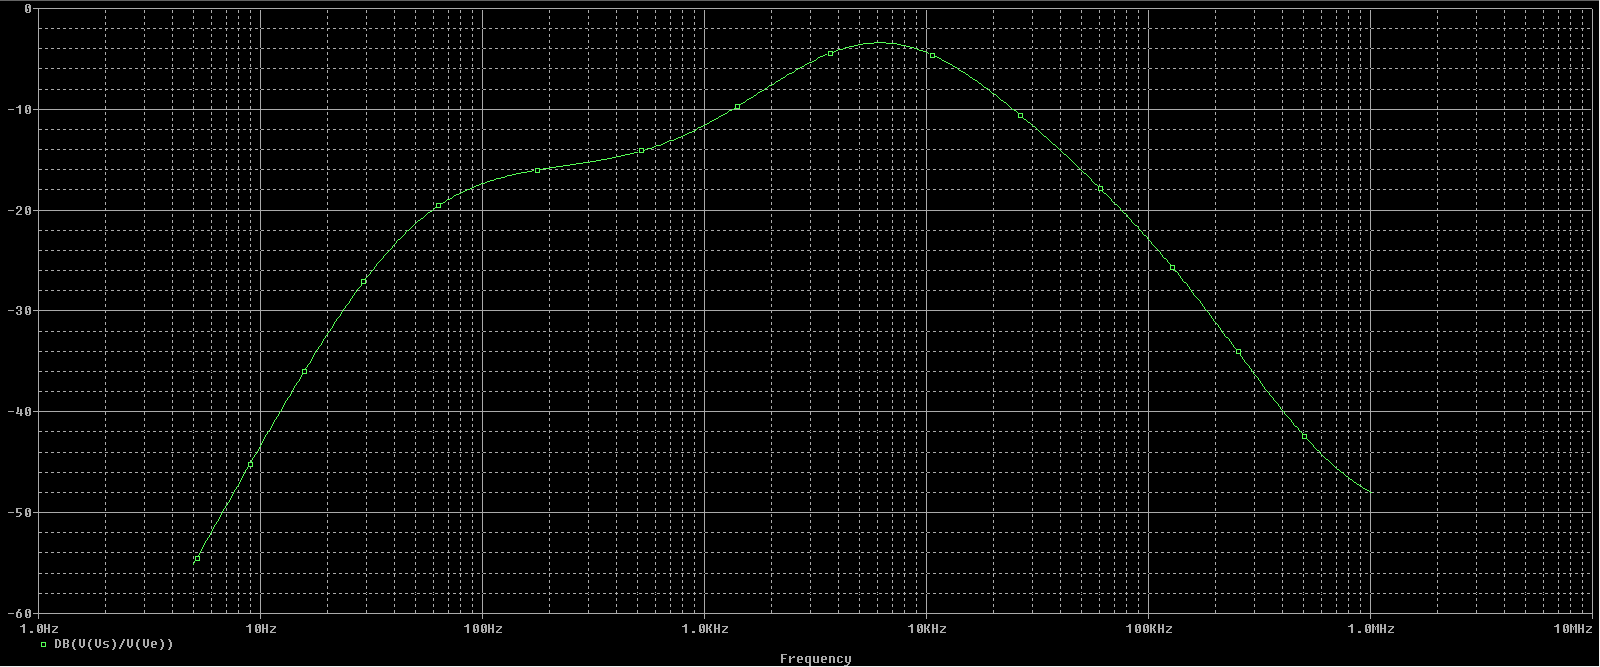
\includegraphics[width=1\textwidth]{Bode_filtre_audio_avec_potentiometre.PNG}
\end{center}

Les fréquences de coupure ainsi que le gain plateau (à 400Hz) sont bien respectés (le gain plateau vaut, à 400Hz : $20log(Avm) \approx -15dB$).

\subsection{Expérimentation du filtre audio}

\begin{center}
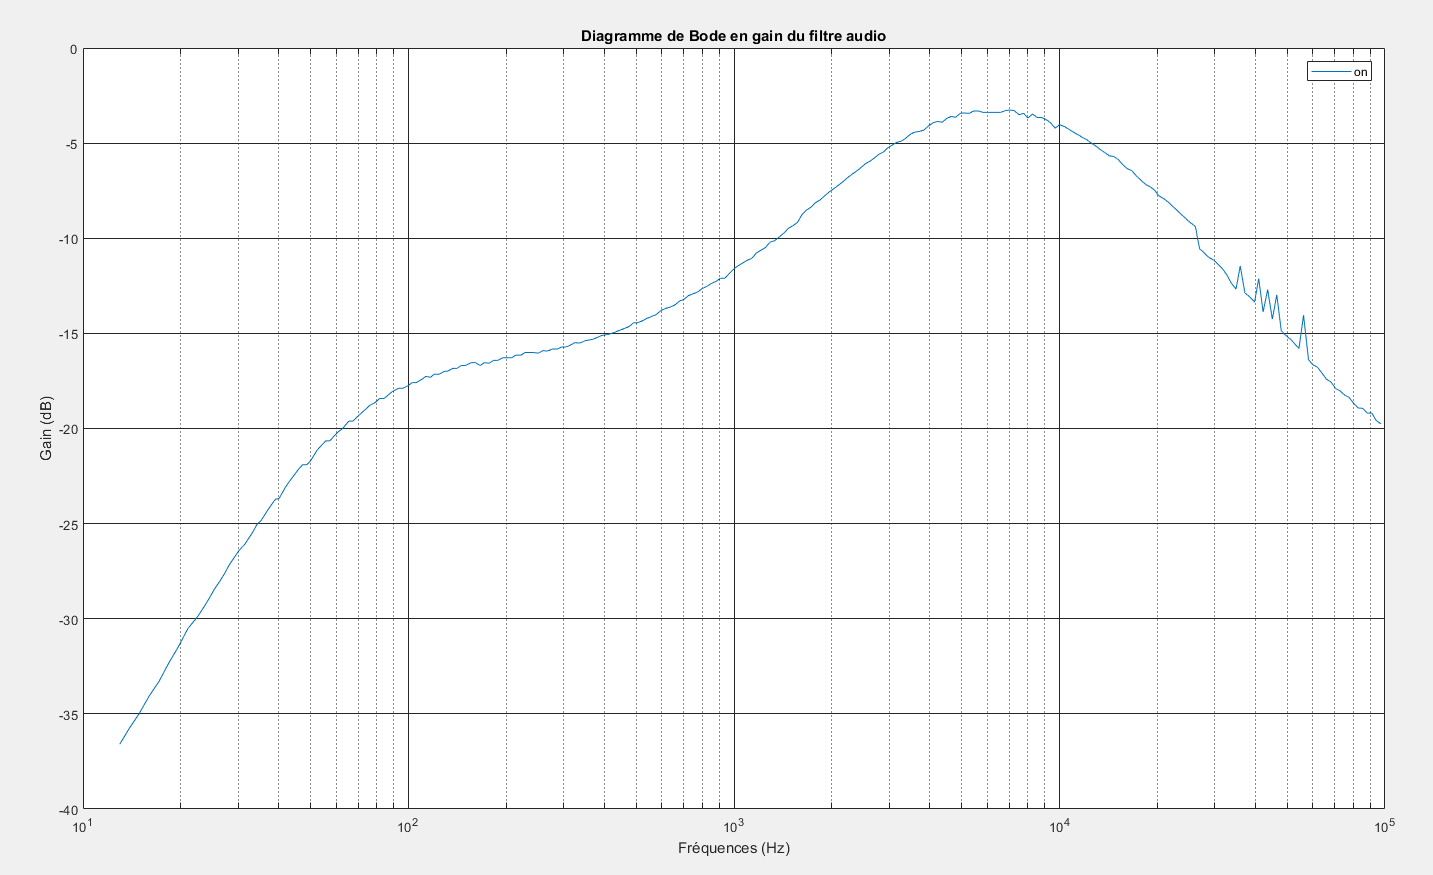
\includegraphics[width=1\textwidth]{Bode_experimental.PNG}
\end{center}

Tout comme pour la simulation, les fréquences de coupure et le gain plateau sont respectés.
\newline

\textbf{\underline{Remarque}} :
\newline
\newline
Pour l'attaque en courant, les fonctions de transfert sont identiques; seul le gain $A_{vm}$ change. Il vaut 0.0928. Ainsi, seule la valeur de $R_5$ change :
$$R_5 = 330\Omega$$.

On obtient le diagramme de Bode suivant sur PSpice :

\begin{center}
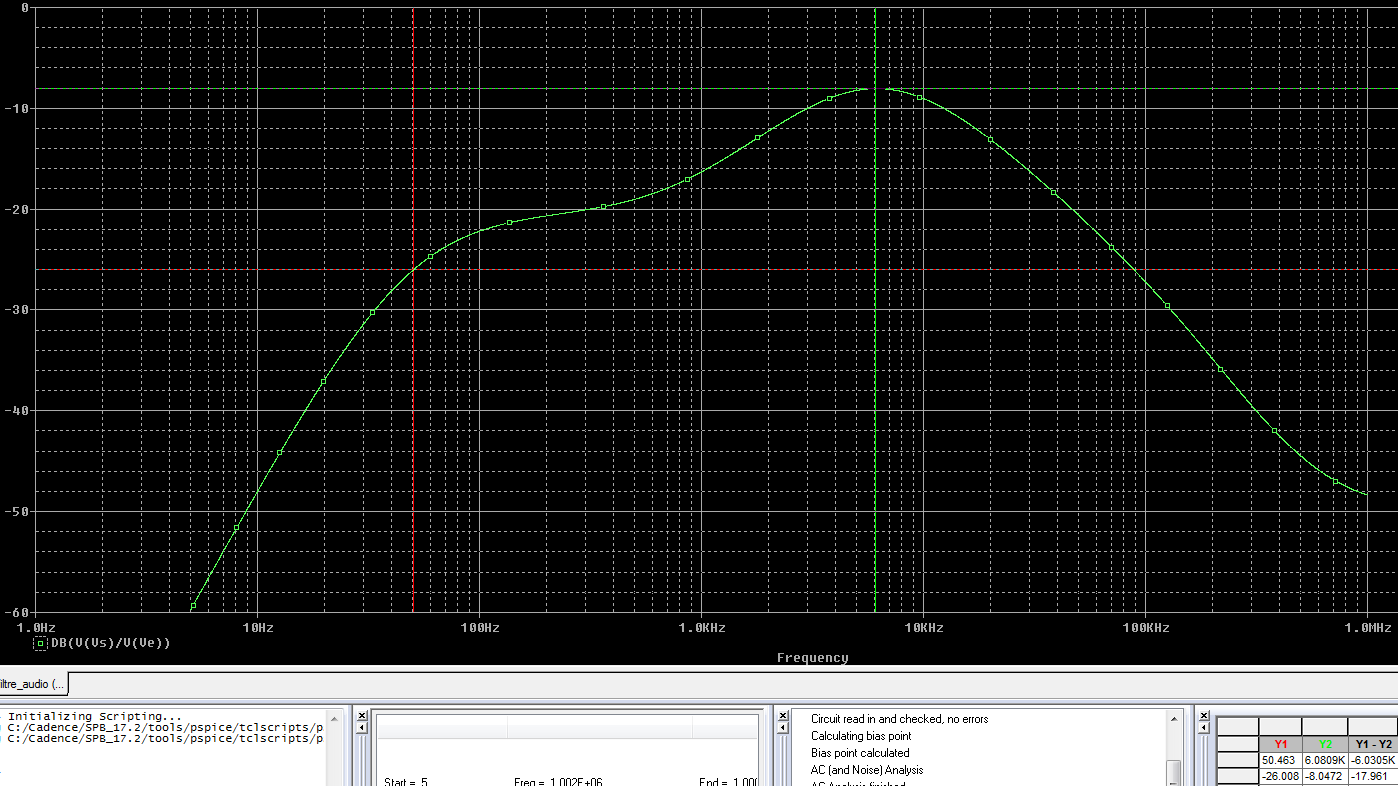
\includegraphics[width=1\textwidth]{bode_filtre.PNG}
\end{center}

Le gain plateau vaut, à 400Hz : $20log(Avm) = -20.6dB$.

\end{document}

% * <man_lot@yahoo.com> 2017-11-13T11:41:30.746Z:
%
% ^.